\documentclass{standalone}
\usepackage{tikz}
\usetikzlibrary{patterns, positioning}
\usepackage[sfdefault]{ClearSans} %% option 'sfdefault' activates Clear Sans as the default text font
\usepackage[T1]{fontenc}

\begin{document}
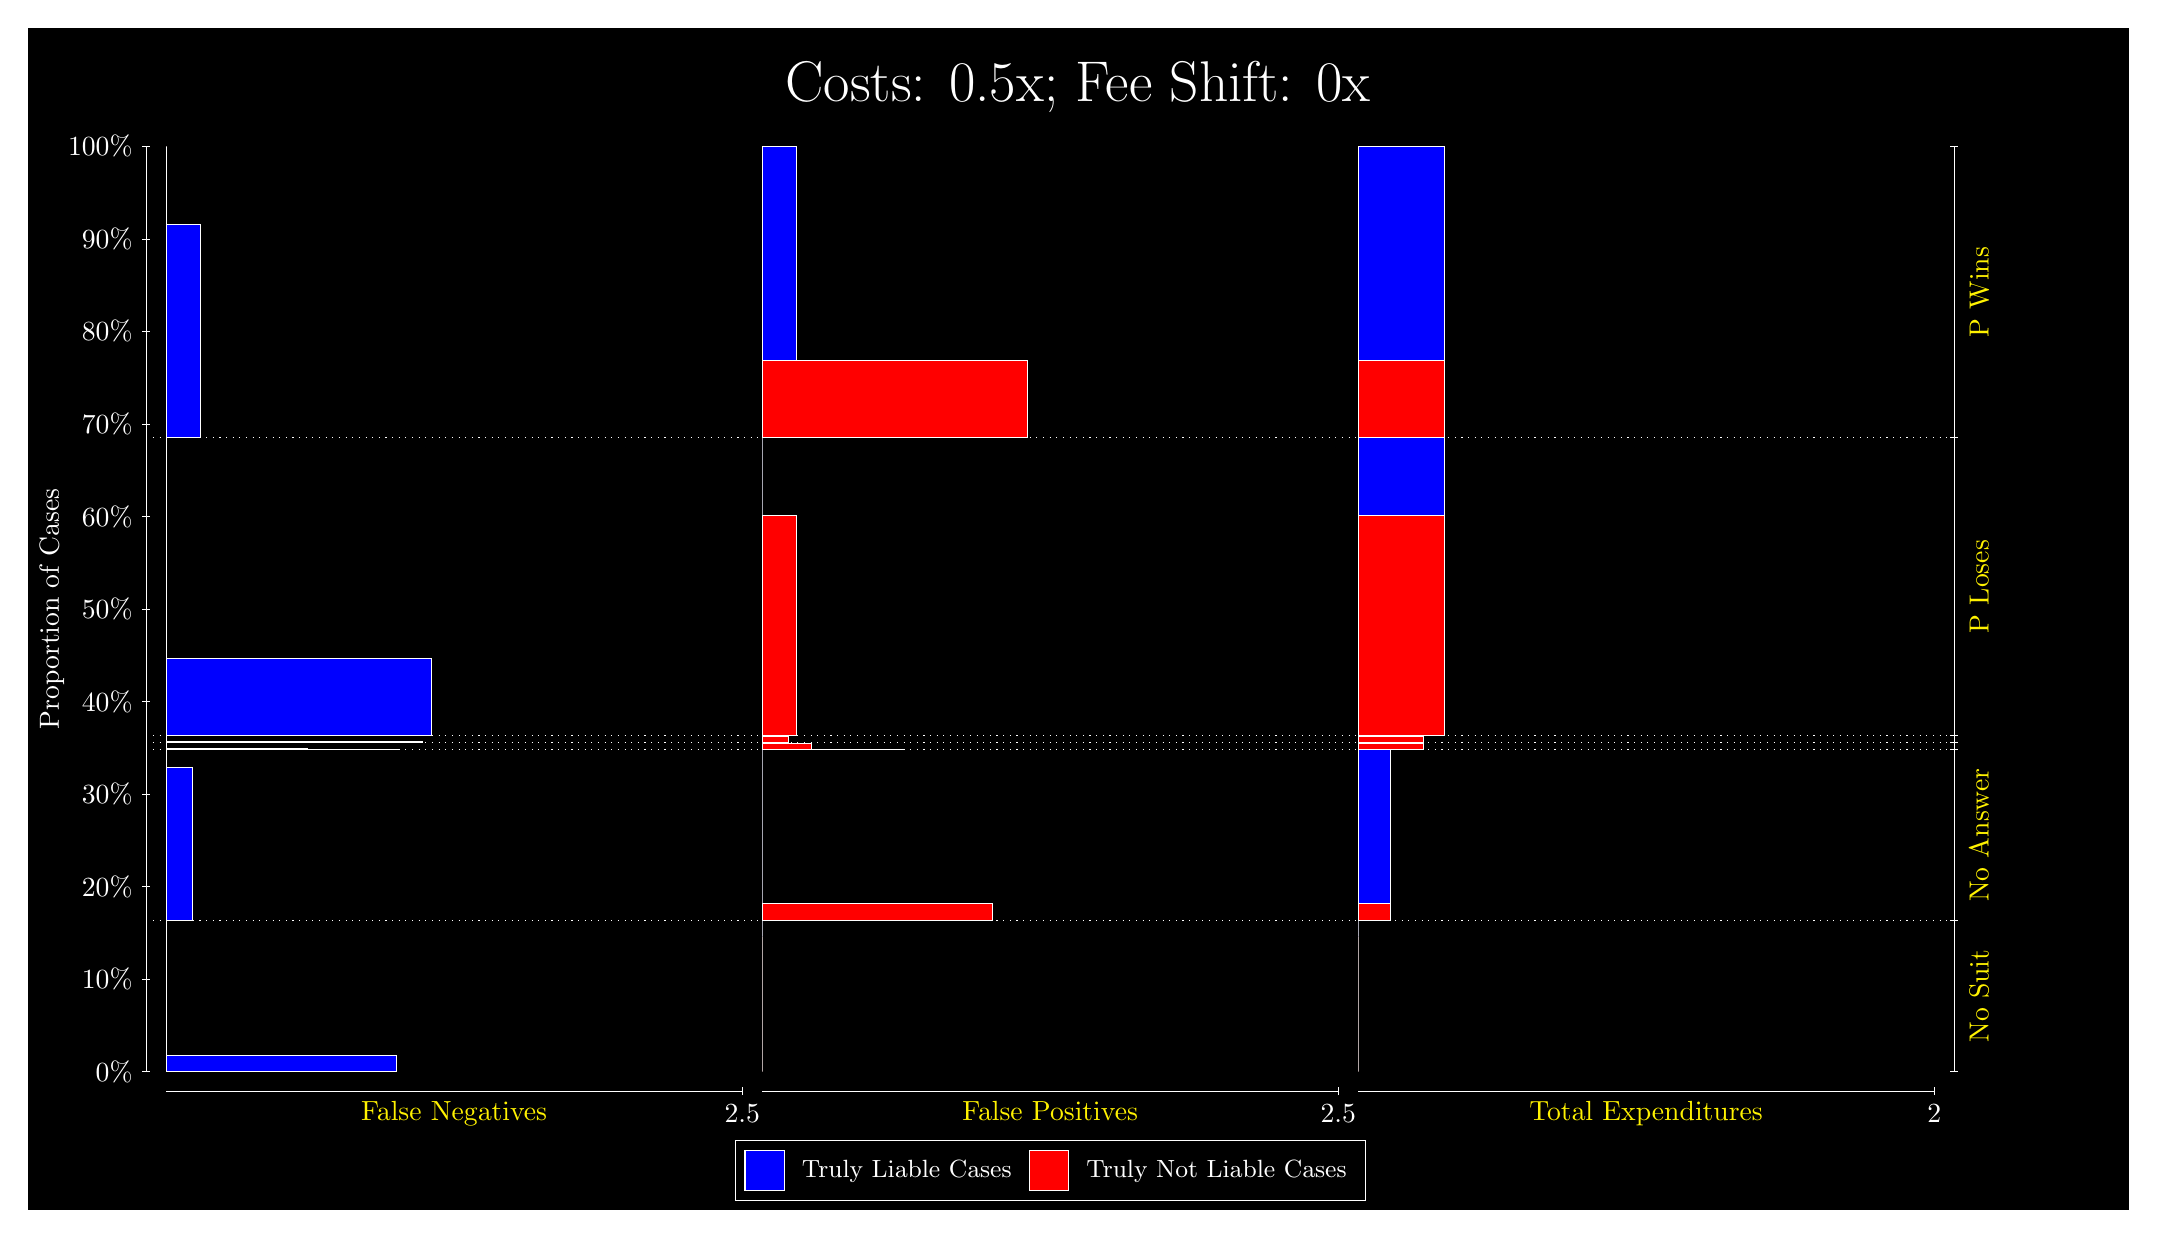
\begin{tikzpicture}
\draw[fill=black] (0,0) rectangle (26.667,15);
\draw[text=white] (0,13.5) rectangle (26.667,15) node[midway] {\huge Costs: 0.5x; Fee Shift: 0x};
\draw[white, very thin] (1.5,1.75) -- (1.5,13.5);
\node[rotate=90, text=white, anchor=center] at (0.3, 7.625) {Proportion of Cases};
\draw[white, very thin] (1.45,1.75) -- (1.55,1.75);
\node[text=white, anchor=east] at (1.45, 1.75) {0\%};
\draw[white, very thin] (1.45,2.925) -- (1.55,2.925);
\node[text=white, anchor=east] at (1.45, 2.925) {10\%};
\draw[white, very thin] (1.45,4.1) -- (1.55,4.1);
\node[text=white, anchor=east] at (1.45, 4.1) {20\%};
\draw[white, very thin] (1.45,5.275) -- (1.55,5.275);
\node[text=white, anchor=east] at (1.45, 5.275) {30\%};
\draw[white, very thin] (1.45,6.45) -- (1.55,6.45);
\node[text=white, anchor=east] at (1.45, 6.45) {40\%};
\draw[white, very thin] (1.45,7.625) -- (1.55,7.625);
\node[text=white, anchor=east] at (1.45, 7.625) {50\%};
\draw[white, very thin] (1.45,8.8) -- (1.55,8.8);
\node[text=white, anchor=east] at (1.45, 8.8) {60\%};
\draw[white, very thin] (1.45,9.975) -- (1.55,9.975);
\node[text=white, anchor=east] at (1.45, 9.975) {70\%};
\draw[white, very thin] (1.45,11.15) -- (1.55,11.15);
\node[text=white, anchor=east] at (1.45, 11.15) {80\%};
\draw[white, very thin] (1.45,12.325) -- (1.55,12.325);
\node[text=white, anchor=east] at (1.45, 12.325) {90\%};
\draw[white, very thin] (1.45,13.5) -- (1.55,13.5);
\node[text=white, anchor=east] at (1.45, 13.5) {100\%};

\draw[white, very thin] (24.457,1.75) -- (24.457,13.5);
\draw[white, very thin] (24.407,1.75) -- (24.507,1.75);
\node[anchor=west] at (24.407, 1.75) {};
\draw[white, very thin] (24.407,3.6646) -- (24.507,3.6646);
\node[anchor=west] at (24.407, 3.6646) {};
\draw[white, very thin] (24.407,5.837) -- (24.507,5.837);
\node[anchor=west] at (24.407, 5.837) {};
\draw[white, very thin] (24.407,5.9312) -- (24.507,5.9312);
\node[anchor=west] at (24.407, 5.9312) {};
\draw[white, very thin] (24.407,6.0165) -- (24.507,6.0165);
\node[anchor=west] at (24.407, 6.0165) {};
\draw[white, very thin] (24.407,9.7986) -- (24.507,9.7986);
\node[anchor=west] at (24.407, 9.7986) {};
\draw[white, very thin] (24.407,13.5) -- (24.507,13.5);
\node[anchor=west] at (24.407, 13.5) {};

\draw[white, very thin, fill=blue] (1.75,1.75) rectangle (4.6775,1.9514);
\draw[white, very thin, fill=red] (1.75,1.9514) rectangle (1.75,3.6646);
\draw[white, very thin, fill=blue] (1.75,3.6646) rectangle (2.0793,5.6139);
\draw[white, very thin, fill=red] (1.75,5.6139) rectangle (1.75,5.837);
\draw[white, very thin, fill=blue] (1.75,5.837) rectangle (4.7141,5.8448);
\draw[white, very thin, fill=blue] (1.75,5.8448) rectangle (4.4214,5.8453);
\draw[white, very thin, fill=blue] (1.75,5.8453) rectangle (4.1286,5.8457);
\draw[white, very thin, fill=blue] (1.75,5.8457) rectangle (3.8359,5.8458);
\draw[white, very thin, fill=blue] (1.75,5.8458) rectangle (3.5431,5.8507);
\draw[white, very thin, fill=red] (1.75,5.8507) rectangle (1.75,5.9312);
\draw[white, very thin, fill=blue] (1.75,5.9312) rectangle (5.0069,5.9398);
\draw[white, very thin, fill=red] (1.75,5.9398) rectangle (1.75,6.0165);
\draw[white, very thin, fill=blue] (1.75,6.0165) rectangle (5.1167,7.0023);
\draw[white, very thin, fill=red] (1.75,7.0023) rectangle (1.75,9.7986);
\draw[white, very thin, fill=blue] (1.75,9.7986) rectangle (2.1891,12.515);
\draw[white, very thin, fill=red] (1.75,12.515) rectangle (1.75,13.5);
\draw[white, very thin, fill=red] (9.3189,1.75) rectangle (9.3189,3.4632);
\draw[white, very thin, fill=blue] (9.3189,3.4632) rectangle (9.3189,3.6646);
\draw[white, very thin, fill=red] (9.3189,3.6646) rectangle (12.246,3.8877);
\draw[white, very thin, fill=blue] (9.3189,3.8877) rectangle (9.3189,5.837);
\draw[white, very thin, fill=red] (9.3189,5.837) rectangle (11.112,5.842);
\draw[white, very thin, fill=red] (9.3189,5.842) rectangle (10.819,5.8422);
\draw[white, very thin, fill=red] (9.3189,5.8422) rectangle (10.526,5.8432);
\draw[white, very thin, fill=red] (9.3189,5.8432) rectangle (10.234,5.8443);
\draw[white, very thin, fill=red] (9.3189,5.8443) rectangle (9.941,5.9175);
\draw[white, very thin, fill=blue] (9.3189,5.9175) rectangle (9.3189,5.9312);
\draw[white, very thin, fill=red] (9.3189,5.9312) rectangle (9.6482,6.0079);
\draw[white, very thin, fill=blue] (9.3189,6.0079) rectangle (9.3189,6.0165);
\draw[white, very thin, fill=red] (9.3189,6.0165) rectangle (9.758,8.8128);
\draw[white, very thin, fill=blue] (9.3189,8.8128) rectangle (9.3189,9.7986);
\draw[white, very thin, fill=red] (9.3189,9.7986) rectangle (12.686,10.784);
\draw[white, very thin, fill=blue] (9.3189,10.784) rectangle (9.758,13.5);
\draw[white, very thin, fill=red] (16.888,1.75) rectangle (16.888,3.4632);
\draw[white, very thin, fill=blue] (16.888,3.4632) rectangle (16.888,3.6646);
\draw[white, very thin, fill=red] (16.888,3.6646) rectangle (17.299,3.8877);
\draw[white, very thin, fill=blue] (16.888,3.8877) rectangle (17.299,5.837);
\draw[white, very thin, fill=red] (16.888,5.837) rectangle (17.711,5.842);
\draw[white, very thin, fill=blue] (16.888,5.842) rectangle (17.711,5.8469);
\draw[white, very thin, fill=red] (16.888,5.8469) rectangle (17.711,5.9222);
\draw[white, very thin, fill=blue] (16.888,5.9222) rectangle (17.711,5.9309);
\draw[white, very thin, fill=red] (16.888,5.9309) rectangle (17.711,5.9311);
\draw[white, very thin, fill=blue] (16.888,5.9311) rectangle (17.711,5.9312);
\draw[white, very thin, fill=red] (16.888,5.9312) rectangle (17.711,6.0079);
\draw[white, very thin, fill=blue] (16.888,6.0079) rectangle (17.711,6.0165);
\draw[white, very thin, fill=red] (16.888,6.0165) rectangle (17.986,8.8128);
\draw[white, very thin, fill=blue] (16.888,8.8128) rectangle (17.986,9.7986);
\draw[white, very thin, fill=red] (16.888,9.7986) rectangle (17.986,10.784);
\draw[white, very thin, fill=blue] (16.888,10.784) rectangle (17.986,13.5);
\draw[white, dotted] (1.5,3.6646) -- (24.457,3.6646);
\draw[white, dotted] (1.5,5.837) -- (24.457,5.837);
\draw[white, dotted] (1.5,5.9312) -- (24.457,5.9312);
\draw[white, dotted] (1.5,6.0165) -- (24.457,6.0165);
\draw[white, dotted] (1.5,9.7986) -- (24.457,9.7986);
\draw[white, very thin] (1.75,1.5) -- (9.0689,1.5);
\node[text=yellow, anchor=north] at (5.4094, 1.5) {False Negatives};
\draw[white, very thin] (9.0689,1.45) -- (9.0689,1.55);
\node[text=white, anchor=north] at (9.0689, 1.45) {2.5};

\draw[white, very thin] (9.3189,1.5) -- (16.638,1.5);
\node[text=yellow, anchor=north] at (12.978, 1.5) {False Positives};
\draw[white, very thin] (16.638,1.45) -- (16.638,1.55);
\node[text=white, anchor=north] at (16.638, 1.45) {2.5};

\draw[white, very thin] (16.888,1.5) -- (24.207,1.5);
\node[text=yellow, anchor=north] at (20.547, 1.5) {Total Expenditures};
\draw[white, very thin] (24.207,1.45) -- (24.207,1.55);
\node[text=white, anchor=north] at (24.207, 1.45) {2};

\node[text=yellow, centered, rotate=90] at (24.777, 2.7073) {No Suit};
\node[text=yellow, centered, rotate=90] at (24.777, 4.7508) {No Answer};


\node[text=yellow, centered, rotate=90] at (24.777, 7.9076) {P Loses};
\node[text=yellow, centered, rotate=90] at (24.777, 11.649) {P Wins};

\draw (12.978300999999998,1.5) node[draw=none] (baseCoordinate) {};
\begin{scope}[align=center]
        \matrix[scale=0.5, draw=white, below=0.5cm of baseCoordinate, nodes={draw}, column sep=0.1cm]{
            \node[rectangle, draw, minimum width=0.5cm, minimum height=0.5cm, fill=blue] {}; &
            \node[draw=none, font=\small, text=white] (B) {Truly Liable Cases}; &
            \node[rectangle, draw, minimum width=0.5cm, minimum height=0.5cm, fill=red] {}; &
            \node[draw=none, font=\small, text=white] (B) {Truly Not Liable Cases}; \\
            };
\end{scope}

\end{tikzpicture}
\end{document}